% env_lib: networked multi-agent control environments with classical and
% learning baselines. Build with ./build.sh (named preprint) or
% ./build.sh --anonymous (anonymous submission version).
\documentclass{article}

\usepackage{microtype}
\usepackage{graphicx}
\usepackage{booktabs}
\usepackage{multirow}
\usepackage{amsmath,amssymb}
\usepackage{xcolor}
\usepackage{listings}
\usepackage{pgfplots}
\pgfplotsset{compat=1.18}
\usepackage{hyperref}
\hypersetup{colorlinks=true,linkcolor=black,citecolor=black,urlcolor=blue!55!black}

% Named preprint by default; build.sh --anonymous removes "accepted".
\providecommand{\icmloptions}{accepted}
\usepackage[\icmloptions]{icmllike}
\usepackage[capitalize,noabbrev]{cleveref}
\renewcommand{\ttdefault}{lmtt}  % narrower than Courier for code and ids
\usepackage{array}

% ---------------------------------------------------------------------------
% Numbers (from the repository's benchmarks and test suite)
% ---------------------------------------------------------------------------
\newcommand{\NumTests}{1{,}419}
\newcommand{\NumIds}{18}
\newcommand{\NumFamilies}{eight}
\newcommand{\repo}{\ificmlshowauthors\url{https://github.com/EricDMW/My_Tool_Box}\else(repository link removed for anonymous review)\fi}

\newcommand{\code}[1]{\texttt{#1}}
\newcommand{\file}[1]{\nolinkurl{#1}}
\newcommand{\envid}[1]{\texttt{#1}}
\lstset{basicstyle=\ttfamily\scriptsize,columns=fullflexible,keepspaces=true,
  frame=single,framerule=0.4pt,rulecolor=\color{black!25},backgroundcolor=\color{black!3},
  xleftmargin=2pt,xrightmargin=2pt,aboveskip=4pt,belowskip=2pt,
  commentstyle=\color{black!55},keywordstyle=\color{blue!55!black},
  stringstyle=\color{green!35!black},showstringspaces=false,language=Python,
  escapeinside={(*}{*)}}

\icmltitlerunning{Networked Multi-Agent Control Environments with Classical and Learning Baselines}

\begin{document}

\twocolumn[
\icmltitle{\texttt{env\_lib}: Networked Multi-Agent Control Environments\\
  with Classical and Learning Baselines}

\icmlsetsymbol{equal}{*}
\begin{icmlauthorlist}
\icmlauthor{Dongming Wang}{ucr}
\end{icmlauthorlist}
\icmlaffiliation{ucr}{University of California, Riverside, CA, USA}
\icmlcorrespondingauthor{Dongming Wang}{wdong025@ucr.edu}
\icmlkeywords{multi-agent reinforcement learning, benchmarks, networked control}

\vskip 0.25in
]

\printAffiliationsAndNotice{}

\begin{abstract}
Cooperative multi-agent reinforcement learning is increasingly proposed for
networked physical systems such as power grids, vehicle platoons and robot
teams, yet many widely used benchmarks are games or particle worlds whose
actions, rewards and scales have no physical meaning, and they rarely tell
the user how far a learned policy is from the controller an engineer would
deploy. We
present \texttt{env\_lib}, a library of {\NumIds} Gymnasium environments in
{\NumFamilies} families of networked multi-agent control problems with
continuous states and actions in physical units: power-grid frequency control,
cooperative adaptive cruise control, consensus and formation control,
oscillator synchronisation, multi-robot localisation and target tracking,
cooperative rigid-body physics, and two discrete networking tasks. All
environments share one interface with joint per-agent spaces, per-agent
rewards and an explicit interaction graph. The continuous environments are
written batch-first, so a vector environment advances all its copies with
array operations: 2.1 to 3.2~million agent-steps per second on one CPU core,
33 to 43 times the throughput of Gymnasium's synchronous vector environment. Every
environment ships a decentralised classical controller as a reference, and a
companion package provides seven multi-agent reinforcement learning baselines
(IPPO, MAPPO, MADDPG, MATD3, IQL, VDN, QMIX) with tuned settings and a
function that compares a new method with all references on identical seeded
episodes.
\end{abstract}

% ===========================================================================
\section{Introduction}
% ===========================================================================

Many engineered systems are collections of agents that act on continuous
physical quantities and interact through a network: generators and inverters
hold the frequency of a transmission grid, vehicles in a platoon keep a safe
gap to their predecessors, and robots share measurements to localise
themselves and a target. Their controllers must be decentralised, because
each agent senses only its neighbourhood, and robust to disturbances.
Multi-agent reinforcement learning (MARL) is a natural candidate for such
problems, and the questions a researcher asks are practical: does the learned
policy stabilise the system, how much control effort does it spend, and does
it beat the classical design?

The standard MARL benchmarks were built for other questions. The particle
environments of \citet{lowe2017maddpg}, the StarCraft challenges
\citep{samvelyan2019smac,ellis2023smacv2}, multi-agent MuJoCo
\citep{peng2021facmac} and the games collected in PettingZoo
\citep{terry2021pettingzoo} have game scores as rewards, discrete or
normalised actions and no notion of a physical operating point. Domain
simulators for power systems \citep{marot2020l2rpn,wang2021mapdn} or traffic
\citep{wu2022flow} are faithful but heavy, each with its own interface. They
rarely ship the reference an engineer would compare against: a classical
controller for the same task, runnable through the same interface.

\texttt{env\_lib} fills this gap with a compact, dependency-light library of
networked control environments. Its contributions are:
\begin{itemize}
  \setlength{\itemsep}{1pt}
  \item {\NumIds} registered environments in {\NumFamilies} families
    (\cref{tab:envs}, \cref{fig:gallery}), from power-grid swing dynamics and
    string-unstable vehicle platoons to discrete networking tasks, all with
    documented dynamics, observation layouts, units and bounds;
  \item one interface across all of them: Gymnasium's API with joint spaces of
    shape \code{(n\_agents, dim)}, per-agent rewards, an explicit interaction
    graph, and adapters to single-agent libraries and to the PettingZoo
    parallel API;
  \item batch-first native vector environments that simulate thousands of
    copies at once on one CPU core, with Gymnasium's autoreset semantics;
  \item a decentralised classical controller for every environment,
    evaluated against random actions on seeded episodes
    (\cref{sec:classical});
  \item seven MARL baselines with tuned settings and a single call that
    compares a new method with random actions, the classical controller and
    the learned baselines on identical episodes (\cref{sec:learning}).
\end{itemize}
The library is open source (MIT licence) at \repo, installs with
\code{pip}, and is covered by {\NumTests} tests and continuous integration on
Python~3.9 to 3.13.

% ===========================================================================
\section{Related Work}
% ===========================================================================

\paragraph{Environment interfaces and suites.} Gym and its successor
Gymnasium \citep{brockman2016gym,towers2024gymnasium} define the single-agent
interface that \texttt{env\_lib} follows; PettingZoo \citep{terry2021pettingzoo}
standardises multi-agent interaction through per-agent dictionaries, which
\texttt{env\_lib} supports through an adapter. The multi-agent particle
environments \citep{lowe2017maddpg}, SMAC and SMACv2
\citep{samvelyan2019smac,ellis2023smacv2} and multi-agent MuJoCo
\citep{peng2021facmac} are the most widely used cooperative benchmarks.
VMAS \citep{bettini2022vmas} vectorises multi-robot scenarios in PyTorch and
JaxMARL \citep{rutherford2024jaxmarl} re-implements popular environments in
JAX for accelerator-scale training. \texttt{env\_lib} shares their emphasis on
batched simulation but targets control problems, runs on NumPy without an
accelerator, and pairs every task with a classical controller.

\paragraph{Domain simulators.} Grid2Op and the L2RPN challenges
\citep{marot2020l2rpn} address topology control of transmission grids, MAPDN
\citep{wang2021mapdn} voltage control in distribution networks, CityLearn
\citep{vazquez2019citylearn} demand response and Flow \citep{wu2022flow}
mixed-autonomy traffic. They model their domains in more detail than
\texttt{env\_lib}, whose environments are deliberately compact models, such as
the swing equations \citep{kundur1994power} or a platoon with actuator lag
\citep{ploeg2011cacc}, that capture the phenomenon a controller must handle and
simulate fast enough for many training runs.

\paragraph{Algorithm libraries.} EPyMARL \citep{papoudakis2021benchmarking},
MARLlib \citep{hu2023marllib} and BenchMARL \citep{bettini2024benchmarl}
provide many algorithms with configurable experiment pipelines. The baselines
of \cref{sec:learning} are deliberately smaller: seven reference
implementations written against the \texttt{env\_lib} interface, with settings
tuned for these environments, meant as ready-made points of comparison.

% ===========================================================================
\section{The Environment Suite}\label{sec:suite}
% ===========================================================================

\begin{table*}[t]
  \caption{The environment families (default configuration). ``Obs.'' is the
    per-agent observation dimension; ``Batch'' marks a native vector
    implementation (the others run in Gymnasium's synchronous or asynchronous
    vector environments). The Kuramoto family treats the network as one agent
    that sets the inputs of all oscillators.}
  \label{tab:envs}
  \centering\footnotesize
  \setlength{\tabcolsep}{3.5pt}
  \renewcommand{\arraystretch}{1.1}
  \begin{tabular}{@{}>{\raggedright}p{3.75cm}>{\raggedright}p{3.25cm}rr>{\raggedright}p{2.1cm}>{\raggedright}p{1.9cm}c>{\raggedright\arraybackslash}p{2.1cm}@{}}
    \toprule
    Id & State and dynamics & Agents & Obs. & Action per agent & Interaction graph & Batch & Classical controller \\
    \midrule
    \envid{PowerGrid-v0} & bus angles and frequencies; swing equations & 16 & 10 & power injection & transmission network & \checkmark & droop control \\
    \envid{Platoon-v0} & gaps, speeds, accelerations; actuator lag & 8 & 13 & acceleration command & V2V topology & \checkmark & CACC \\
    \envid{Consensus-v0}, \envid{Formation-v0} & planar positions; single or double integrator & 8 & 16 & 2-D velocity & ring or proximity & \checkmark & Laplacian protocol \\
    \envid{KuramotoOscillator-*} (4 ids) & phases; coupled oscillators & 1 & 18--75 & inputs, coupling gains & coupling matrix & \checkmark & phase feedback \\
    \envid{KuramotoOscillatorTorch-*} (5 ids) & the same on PyTorch tensors & 1 & 18--75 & inputs, coupling gains & coupling matrix & tensors & phase feedback \\
    \envid{AJLATT-v0} & poses and EKF beliefs; unicycles & 4 & 24 & linear, angular velocity & sensing range & & encircle target belief \\
    \envid{Pistonball-v0} & ball and pistons; rigid bodies & 20 & 7 & piston velocity & adjacent pistons & & ramp towards ball \\
    \envid{LineMsg-v0} & message states; lossy links & 10 & 3 & relay or not & line & & always relay \\
    \envid{WirelessComm-v0}, \envid{-v1} & packet queues; shared access points & 36, 16 & 18 & idle or one of 4 APs & grid & & collision-free schedule \\
    \bottomrule
  \end{tabular}
\end{table*}

\begin{figure*}[t]
  \centering
  \setlength{\tabcolsep}{2pt}
  \begin{tabular}{cccc}
    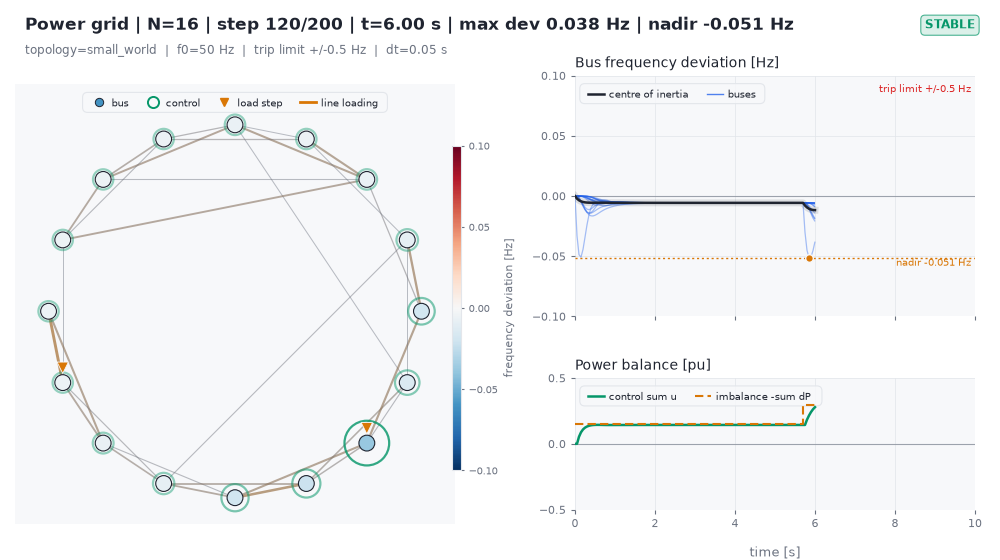
\includegraphics[width=0.24\textwidth,height=2.4cm,keepaspectratio]{figures/power_grid.png} &
    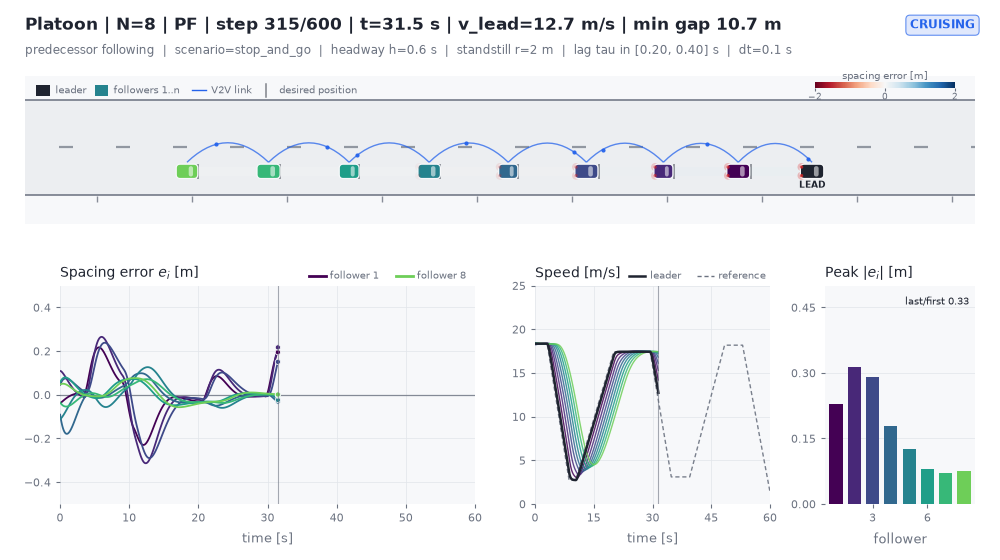
\includegraphics[width=0.24\textwidth,height=2.4cm,keepaspectratio]{figures/platoon.png} &
    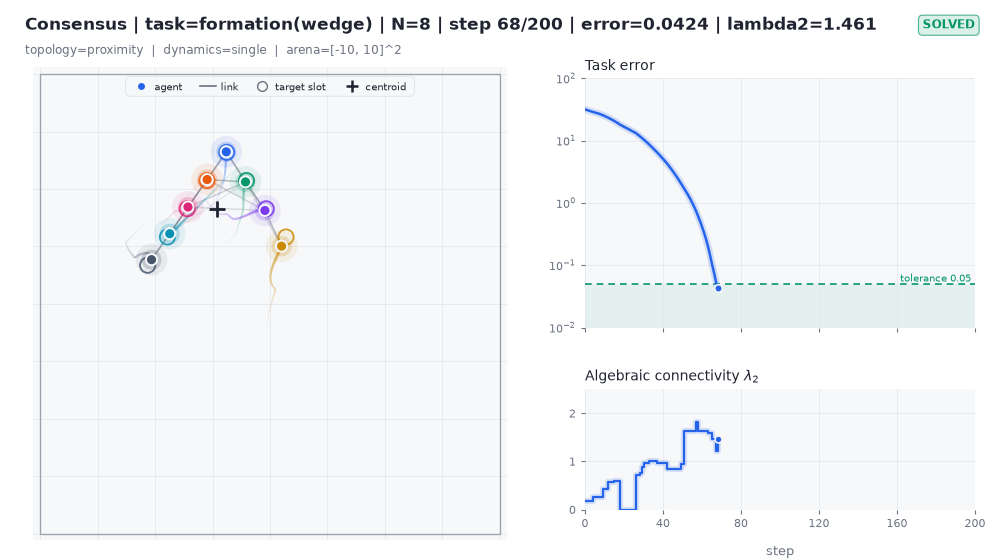
\includegraphics[width=0.24\textwidth,height=2.4cm,keepaspectratio]{figures/formation.png} &
    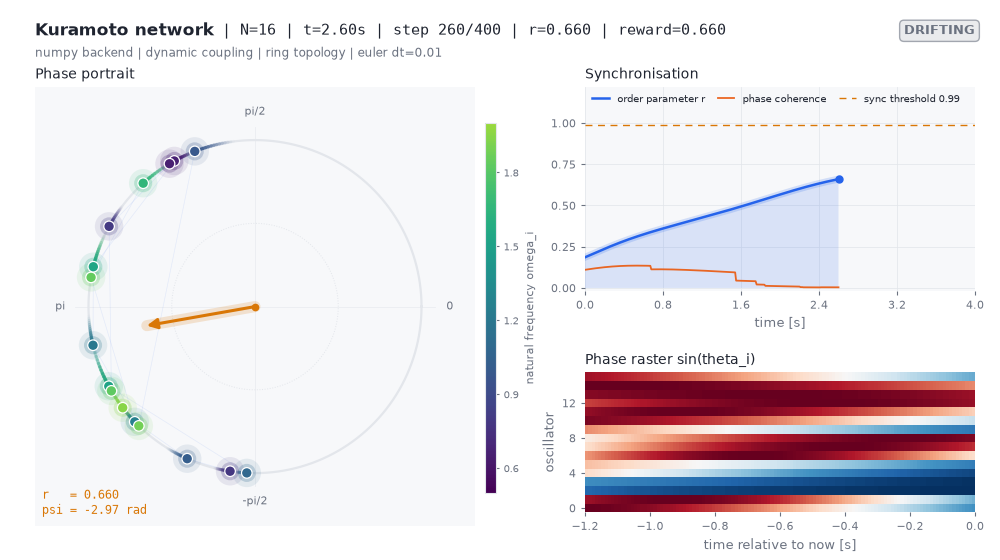
\includegraphics[width=0.24\textwidth,height=2.4cm,keepaspectratio]{figures/kuramoto.png} \\[-1pt]
    {\scriptsize \envid{PowerGrid-v0}} & {\scriptsize \envid{Platoon-v0}} &
    {\scriptsize \envid{Formation-v0}} & {\scriptsize \envid{KuramotoOscillator-v0}} \\[2pt]
    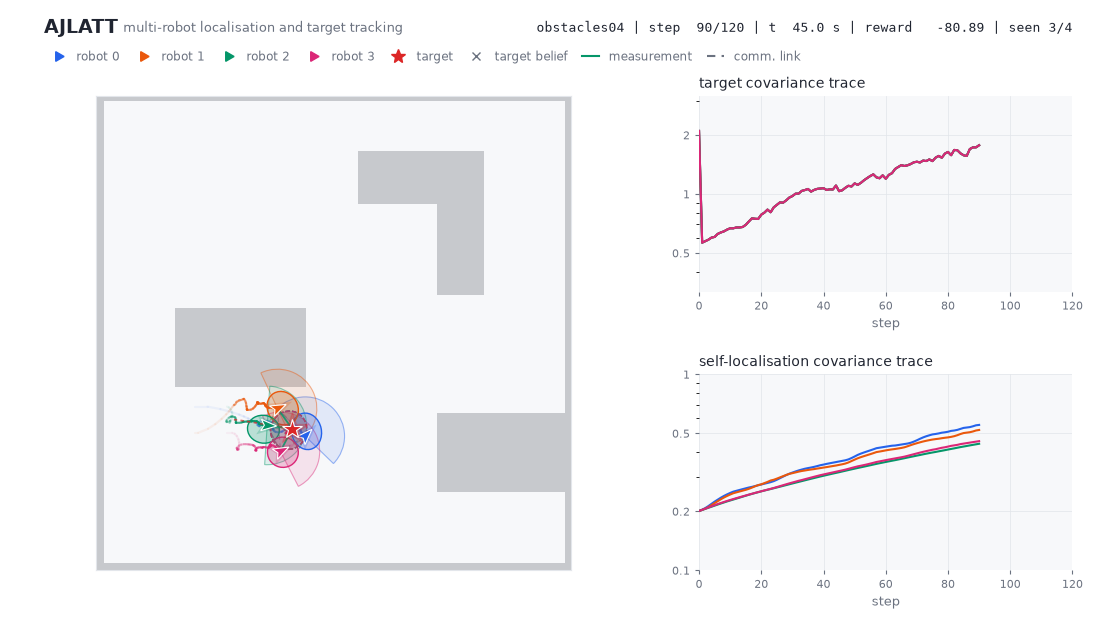
\includegraphics[width=0.24\textwidth,height=2.4cm,keepaspectratio]{figures/ajlatt.png} &
    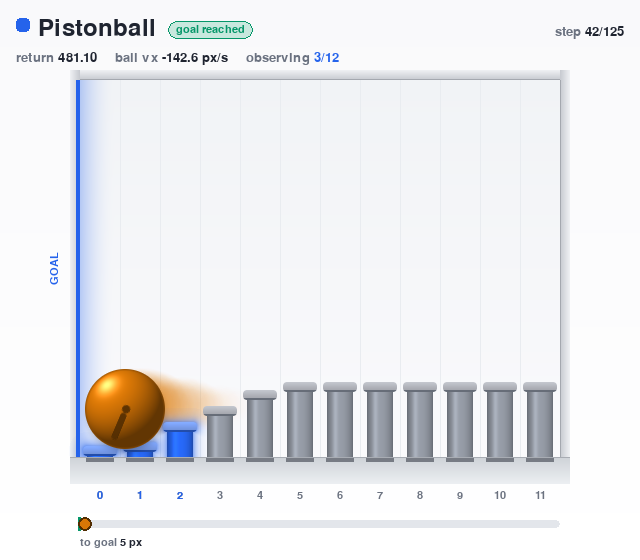
\includegraphics[width=0.24\textwidth,height=2.4cm,keepaspectratio]{figures/pistonball.png} &
    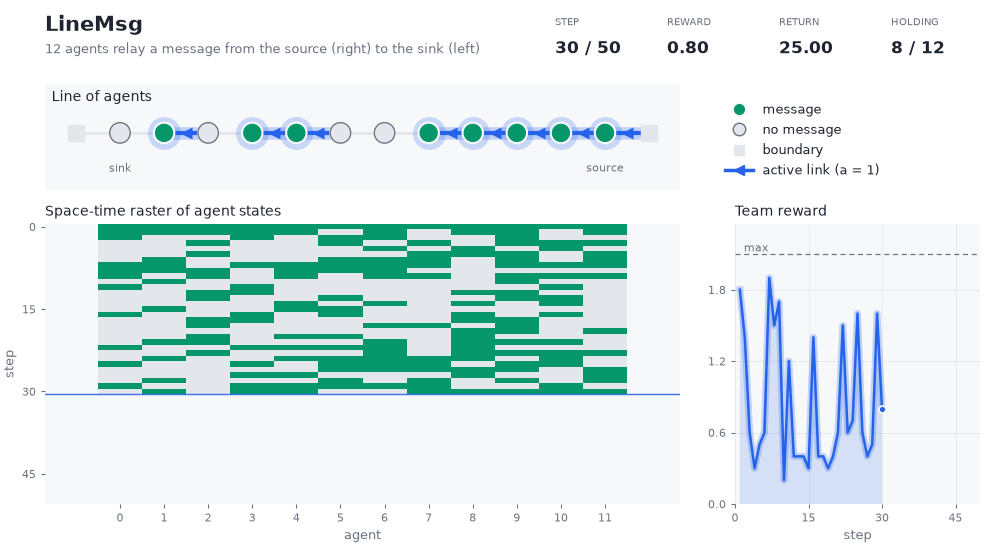
\includegraphics[width=0.24\textwidth,height=2.4cm,keepaspectratio]{figures/linemsg.png} &
    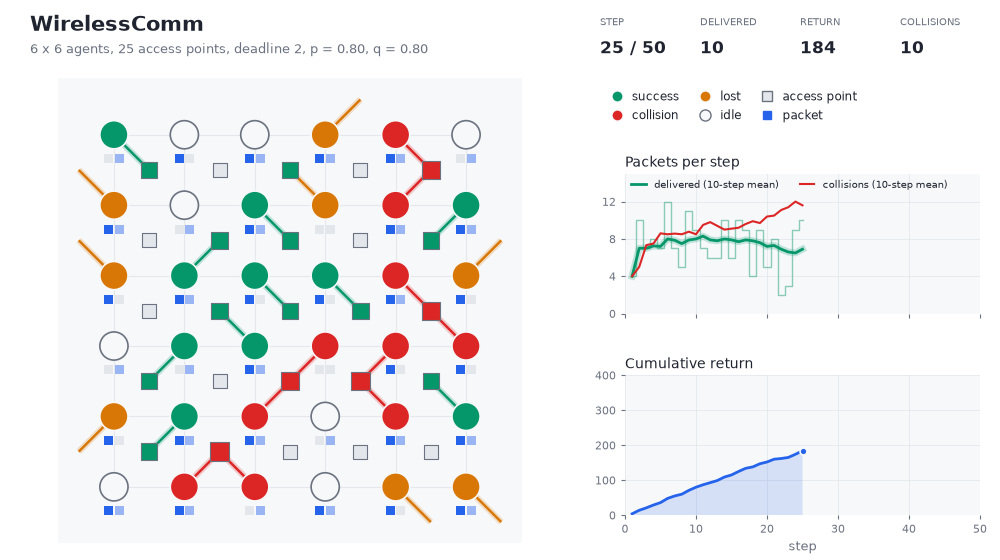
\includegraphics[width=0.24\textwidth,height=2.4cm,keepaspectratio]{figures/wireless.png} \\[-1pt]
    {\scriptsize \envid{AJLATT-v0}} & {\scriptsize \envid{Pistonball-v0}} &
    {\scriptsize \envid{LineMsg-v0}} & {\scriptsize \envid{WirelessComm-v1}} \\
  \end{tabular}
  \caption{Frames rendered by \code{env.render()} in \code{"rgb\_array"} mode.
    Each frame is a dashboard: the system state next to time series of the
    quantities that matter for the task (frequencies, spacing errors,
    disagreement, order parameter, estimation uncertainty, deliveries).}
  \label{fig:gallery}
\end{figure*}

\subsection{A Common Interface}\label{sec:interface}

Every environment follows the Gymnasium API \citep{towers2024gymnasium}.
Observations and actions of multi-agent environments are joint: an
observation has shape \code{(n\_agents, obs\_dim)}, one row per agent, and an
action \code{(n\_agents, action\_dim)} or \code{(n\_agents,)}. \code{step}
returns the team reward, and the individual rewards are in
\code{info["agent\_rewards"]}, so that both cooperative (team) and
individual-reward learning are possible without wrappers. \code{terminated}
signals a task outcome (a trip, a collision, synchronisation reached) and
\code{truncated} the environment's own step limit. All randomness comes from
the seeded generator of the environment, so a seed fixes the episode.

Observations are local: each row contains only what the agent could measure
or receive from its neighbours. Every networked environment exposes its
interaction graph as \code{env.adjacency}. The features of an observation row
are documented, scaled to order one, and listed at run time by the properties
\code{observation\_layout} and \code{observation\_scale}. Registered ids come with a catalogue
(\code{env\_lib.catalog()} and the \code{env-lib list} command) that reports
agents, spaces, optional requirements and whether a native vector
implementation exists. One environment deviates from the joint reward
convention for historical reasons: \envid{AJLATT-v0} returns per-robot reward
and termination arrays; a \code{TeamReward} wrapper, applied automatically by
\code{env\_lib.make\_vec}, converts it.

\subsection{The Environments}\label{sec:envs}

\paragraph{Power-grid frequency control.} In \envid{PowerGrid-v0}, bus $i$ of
a Kron-reduced, lossless transmission network has angle $\theta_i$ and
frequency deviation $\omega_i$, governed by the swing equations
\citep{kundur1994power,dorfler2013smartgrids}
\begin{align}
  \dot\theta_i &= \omega_i, \nonumber\\
  M_i \dot\omega_i &= P_i(t) - D_i\omega_i
    - \textstyle\sum_j B_{ij}\sin(\theta_i-\theta_j) + u_i,
\end{align}
with heterogeneous inertia $M_i$ and damping $D_i$, line susceptances
$B_{ij}$ on a small-world graph of 16 buses, step load changes and optional
load noise in $P_i(t)$, and a bounded fast frequency response
$u_i \in [-u_{\max,i}, u_{\max,i}]$ as the action. Every episode starts from an
exact, stable equilibrium with a prescribed line loading. Agents are penalised
for frequency deviation, rate of change of frequency and control effort; a
frequency beyond 0.5\,Hz trips the system and ends the episode. Episodes last
10\,s (200 steps).

\paragraph{Vehicle platoon.} In \envid{Platoon-v0}, a leader drives an
exogenous speed profile (cruising, stop-and-go waves, random changes) and
eight followers command their accelerations through a first-order actuator
lag, $\dot a_i = (u_i - a_i)/\tau_i$, discretised exactly. Each follower keeps
a constant time headway, $e_i = g_i - (r + h v_i)$, and observes what its
vehicle-to-vehicle topology provides (predecessor, predecessor and leader,
bidirectional, or sensors only). The environment reproduces the central
phenomenon of platoon control, string instability
\citep{swaroop1996string,naus2010cacc}: with sensor-only cruise control and a
short headway, spacing errors grow along the platoon until vehicles collide.
Rewards penalise spacing and speed errors, control and jerk; a collision or a
break-up ends the episode (600 steps of 0.1\,s).

\paragraph{Consensus and formation.} In \envid{Consensus-v0} and
\envid{Formation-v0}, eight agents with single- or double-integrator dynamics in a bounded plane
must agree on a position (rendezvous) or on a shape, with shifted positions
$y_i = x_i - d_i$ for formation offsets $d_i$. They communicate over a static
graph (a ring by default; line, star, complete or Erd\H{o}s--R\'enyi) or a
proximity graph that changes as they move, and each agent is penalised by its mean
squared disagreement with its neighbours and its control effort
\citep{olfati2004consensus,olfati2007consensus}.

\paragraph{Oscillator synchronisation.} In the Kuramoto family, the phases
follow the controlled Kuramoto model
$\dot\theta_i = \omega_i + a_i + c\sum_j K_{ij}\sin(\theta_j-\theta_i)$
\citep{kuramoto1984chemical,dorfler2014survey}, integrated with Euler or
Runge--Kutta steps. The controller sets the inputs $a_i$ and, in the dynamic
coupling mode, the coupling gains; rewards are the order parameter, the phase
coherence or the frequency-tracking error. A PyTorch backend simulates batches
of systems on a CPU or GPU.

\paragraph{Multi-robot localisation and target tracking.} In
\envid{AJLATT-v0}, four unicycle robots without absolute positioning estimate their own poses
and the pose of a moving target with extended Kalman filters, from noisy
range--bearing measurements that obstacles on an occupancy map can block, and
fuse neighbours' estimates by covariance intersection
\citep{julier1997ci}. The reward penalises the traces of the robots' own and
target covariances and collisions, so the team must move to keep the target
observed while staying localised.

\paragraph{Pistonball.} Twenty pistons move a ball to
the left wall in a rigid-body simulation (pymunk), a cooperative game
popularised by PettingZoo \citep{terry2021pettingzoo}, here re-implemented with
the joint interface, local rewards within a configurable neighbourhood,
continuous or discrete actions and a keyboard mode.

\paragraph{Discrete networked tasks.} In \envid{LineMsg-v0}, agents on a line
relay a message from a source to a sink over lossy links; relaying keeps a
link active, and the team is rewarded for holding and delivering the message.
In \envid{WirelessComm-v0} and \envid{-v1}, agents on a $6\times6$ or
$4\times4$ grid hold packet queues with deadlines and transmit to one of up to
four shared access points; a transmission succeeds only if no other agent
uses the same access point, in the spirit of the wireless multiple-access
problems studied for scalable networked reinforcement learning
\citep{qu2020scalable}. Both expose a credit-assignment problem: in
WirelessComm a collision costs the transmitting agent nothing under its own
reward.

% ===========================================================================
\section{Using the Environments}\label{sec:usage}
% ===========================================================================

\subsection{Single Environments and Batches}

\Cref{lst:basic} shows the complete workflow. \code{env\_lib.make} creates an
environment by id with keyword overrides of any constructor argument;
\code{env\_lib.make\_vec(id, num\_envs)} returns the native batched
implementation where one exists and Gymnasium's synchronous vector
environment otherwise (\code{vectorization\_mode="async"} selects the
asynchronous one). Native vector environments support Gymnasium's three
autoreset modes and a reset mask, and every copy reproduces the single
environment started from the same state, which the test suite checks.

\begin{lstlisting}[caption={Create, control, batch and evaluate.},label={lst:basic},captionpos=b,float=t]
import env_lib

env = env_lib.make("PowerGrid-v0")   # kwargs override
obs, info = env.reset(seed=0)        # (16, 10) float32
ctrl = env_lib.baseline_policy(env)  # droop control
obs, r, term, trunc, info = env.step(ctrl(obs))
info["agent_rewards"]                # shape (16,)

envs = env_lib.make_vec("PowerGrid-v0", 1024)
res = env_lib.evaluate(envs, ctrl, n_episodes=1024,
                       seed=0)       # about one second
print(res.mean_return, res.ci95)
\end{lstlisting}

\subsection{Evaluation}

\code{env\_lib.evaluate(env, policy, n\_episodes, seed)} runs a policy on a
single or vector environment and returns the episode returns with their mean,
standard deviation and 95\,\% confidence interval, episode lengths and
per-agent returns. \code{policy=None} samples uniformly random actions from a
seeded copy of the action space. On a vector environment every copy
contributes the first episodes it finishes, handling all autoreset modes, so
random actions, a controller and a learned policy evaluated with the same seed
meet the same initial conditions and disturbances.

\subsection{Interoperability and Command Line}

Two wrappers connect the joint interface to existing learners:
\code{FlattenJointSpaces} flattens joint spaces for single-agent libraries,
and \code{to\_parallel(id)} exposes an environment through the PettingZoo
parallel API with per-agent dictionaries, which passes PettingZoo's API test.
The \code{env-lib} command runs the most common tasks without code:
\begin{lstlisting}[language=bash]
env-lib list --continuous     # the catalogue
env-lib describe Platoon-v0   # spaces, layout
env-lib run Formation-v0 --gif run.gif
env-lib evaluate PowerGrid-v0 --episodes 64 \
                              --num-envs 64
env-lib bench Platoon-v0 --num-envs 1024
\end{lstlisting}

\subsection{Performance}\label{sec:performance}

The continuous environments implement their dynamics once, for arrays with a
leading batch axis; the single environment is the batch of one. A vector
environment therefore advances all copies with a few array operations instead
of a Python loop over copies. \Cref{tab:throughput} and \cref{fig:throughput}
report the throughput on one core of an Intel Xeon at 2.8\,GHz with random
actions and automatic resets included: 2.1 to 3.2~million agent-steps per
second at 256 copies, 33 to 43 times Gymnasium's \code{SyncVectorEnv}, whose
throughput stays at a few thousand steps per second whatever the batch size.
Rendering is independent of simulation and only runs when requested.

\begin{table}[t]
  \caption{Environment steps per second on one CPU core, random actions,
    automatic resets included (\file{benchmarks/benchmark_vector.py}).}
  \label{tab:throughput}
  \centering\small
  \setlength{\tabcolsep}{3.5pt}
  \begin{tabular}{@{}lrrrrr@{}}
    \toprule
    & & & \multicolumn{2}{c}{256 copies} & \\
    \cmidrule(lr){4-5}
    Environment & $n$ & 1 copy & native & Sync & speed-up \\
    \midrule
    PowerGrid & 16 & 3.3k & 134k & 3.1k & 43$\times$ \\
    Platoon & 8 & 7.1k & 295k & 7.4k & 40$\times$ \\
    Consensus & 8 & 7.9k & 345k & 8.7k & 40$\times$ \\
    Formation & 8 & 7.9k & 313k & 8.3k & 38$\times$ \\
    Kuramoto & 10 & 6.9k & 316k & 9.6k & 33$\times$ \\
    \bottomrule
  \end{tabular}
\end{table}

\begin{figure}[t]
  \centering
  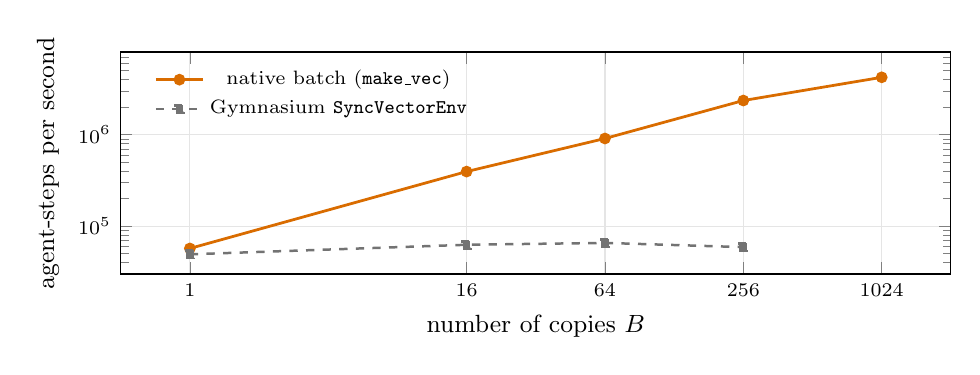
\begin{tikzpicture}
    \begin{loglogaxis}[width=\columnwidth,height=4.4cm,
        xlabel={number of copies $B$},ylabel={agent-steps per second},
        xtick={1,16,64,256,1024},xticklabels={1,16,64,256,1024},
        ymin=3e4,ymax=8e6,legend pos=north west,legend style={font=\scriptsize,draw=none,fill=none},
        tick label style={font=\scriptsize},label style={font=\small},grid=major,
        grid style={black!10}]
      \addplot[color=orange!85!black,mark=*,mark size=1.6pt,line width=1pt]
        coordinates {(1,57023) (16,394933) (64,908170) (256,2361407) (1024,4235400)};
      \addlegendentry{native batch (\code{make\_vec})}
      \addplot[color=black!55,mark=square*,mark size=1.4pt,dashed,line width=0.9pt]
        coordinates {(1,49192) (16,62560) (64,65584) (256,58960)};
      \addlegendentry{Gymnasium \code{SyncVectorEnv}}
    \end{loglogaxis}
  \end{tikzpicture}
  \caption{Throughput of \envid{Platoon-v0} (8 followers) on one CPU core as
    a function of the batch size.}
  \label{fig:throughput}
\end{figure}

% ===========================================================================
\section{Integrated Baselines}\label{sec:baselines}
% ===========================================================================

\subsection{Classical Controllers}\label{sec:classical}

\code{env\_lib.baseline\_policy(env)} returns a decentralised classical
controller for every environment: a pure function of the observation, so the
same call drives a single environment or a batch of thousands, and its gains
are keyword arguments. The controllers are the standard designs of each field:
droop control $u_i = -k\,\omega_i$ for the grid, cooperative adaptive cruise
control $u_i = k_p e_i + k_d (v_{i-1}-v_i) + k_a a_{i-1}$ with string-stable
default gains for the platoon \citep{ploeg2011cacc}, the Laplacian protocol
$u_i = k\sum_{j\in\mathcal{N}_i}(y_j-y_i)$ for consensus and formation
\citep{olfati2004consensus}, frequency compensation with mean-field phase
feedback for the oscillators, a formation around the target belief for
AJLATT, a ramp towards the ball for Pistonball, ``always relay'' for LineMsg
(the optimal policy) and a collision-free access schedule for WirelessComm.

\Cref{tab:controllers} compares them with random actions. Two tasks need care
when reading returns. The Kuramoto environments with an order-parameter reward
pay a positive reward per step and end on synchronisation, so the controller,
which synchronises in half the steps, collects less; their task metric is the
time to synchronise. The default AJLATT episode ends at the first collision,
which rewards random robots for colliding early, so the table uses the variant
without collision termination. A learner can exploit both designs by ending
episodes early; \code{env-lib describe} flags them, and for training we
recommend a larger synchronisation bonus or the frequency-tracking reward,
and AJLATT with \code{terminate\_on\_collision=False}.

\begin{table}[t]
  \caption{Mean return of uniformly random actions and the classical
    controller on the same 64 seeded episodes (one per copy of a
    64-copy vector environment, seed 0; \file{benchmarks/benchmark_baselines.py}).
    Higher is better. $^\dagger$Episode length in parentheses; the episode ends on
    synchronisation. $^\ddagger$Without collision termination.}
  \label{tab:controllers}
  \centering\small
  \setlength{\tabcolsep}{3pt}
  \begin{tabular}{@{}llrr@{}}
    \toprule
    Environment & Controller & Random & Controller \\
    \midrule
    PowerGrid & droop & $-562.1$ & $-0.76$ \\
    Platoon & CACC & $-5{,}604$ & $-46.3$ \\
    Consensus & Laplacian & $-17{,}327$ & $-1{,}414$ \\
    Formation & Laplacian & $-18{,}166$ & $-1{,}608$ \\
    Kuramoto-v0$^\dagger$ & phase feedback & 24.0 (21) & 17.2 (10) \\
    Kuramoto freq.\ sync & phase feedback & $-128.1$ & $-112.0$ \\
    AJLATT$^\ddagger$ & encircle & $-34{,}273$ & $-7{,}415$ \\
    Pistonball & ramp & $-253.7$ & 801.3 \\
    LineMsg & always relay & 42.7 & 95.0 \\
    WirelessComm-v0 & schedule & 388.0 & 923.8 \\
    WirelessComm-v1 & schedule & 140.5 & 339.4 \\
    \bottomrule
  \end{tabular}
\end{table}

\begin{figure*}[t]
  \centering
  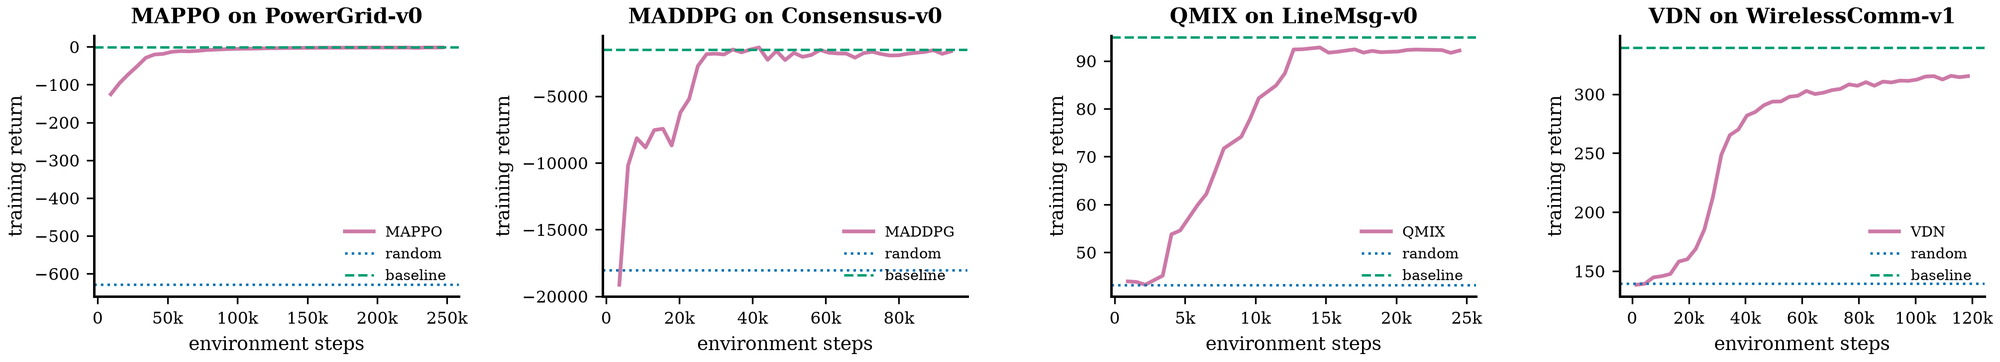
\includegraphics[width=\textwidth]{figures/marl_training.png}
  \caption{Training return of one method of each family with its preset,
    against the evaluation returns of random actions and the classical
    controller (\file{examples/algorithms/marl_training_demo.py}).}
  \label{fig:curves}
\end{figure*}

\subsection{Learning Baselines}\label{sec:learning}

The companion package \texttt{marl\_algorithms} implements seven widely used
cooperative MARL methods against one small core
(\cref{tab:algorithms}): independent and multi-agent PPO
\citep{schulman2017ppo,dewitt2020ippo,yu2022mappo} with generalised advantage
estimation \citep{schulman2016gae}, MADDPG and MATD3
\citep{lowe2017maddpg,ackermann2019matd3} with centralised critics, and
independent Q-learning, VDN and QMIX
\citep{tan1993iql,mnih2015dqn,sunehag2018vdn,rashid2018qmix}. All collect
experience from the native vector environments, act from local observations
(centralised information is used only in training), share or separate
parameters across agents, save and load, and evaluate through
\code{env\_lib.evaluate}. Standard simplifications are stated in the code:
feed-forward networks, a transition replay for the value-based methods, and
the concatenated observations as the global state.

\begin{table}[t]
  \caption{The learning baselines.}
  \label{tab:algorithms}
  \centering\small
  \setlength{\tabcolsep}{3pt}
  \begin{tabular}{@{}lll@{}}
    \toprule
    Method & Family & Idea \\
    \midrule
    IPPO & on-policy & PPO per agent, own reward \\
    MAPPO & on-policy & centralised critic $V(s, i)$ \\
    MADDPG & off-policy & deterministic actors, critics $Q_i(s, a)$ \\
    MATD3 & off-policy & twin critics, target smoothing \\
    IQL & value-based & independent DQN per agent \\
    VDN & value-based & $Q_{\mathrm{tot}} = \sum_i Q_i$ \\
    QMIX & value-based & monotonic mixing conditioned on $s$ \\
    \bottomrule
  \end{tabular}
\end{table}

Seventeen tuned presets pair the methods with the environments whose action
type they support; each trains in under two minutes on one CPU core.
\Cref{tab:marl} lists representative results and \cref{fig:curves} learning
curves (all 17 in \cref{app:presets}). Every learned policy but one closes at
least 98\,\% of the gap between random actions and the classical controller;
the exception, QMIX on WirelessComm, closes 90\,\%. All methods match the optimal relay on
LineMsg, and VDN comes within 0.5\,\% of the collision-free schedule on
WirelessComm; on the continuous tasks the classical controllers remain
ahead, which makes these environments a demanding test for new methods.
Independent Q-learning does not learn WirelessComm at all (152 after the VDN
budget): under per-agent rewards a collision costs the sender nothing, while
VDN and QMIX, trained on the team reward, learn to leave contested access
points to one agent.

\begin{table}[t]
  \caption{Tuned presets: mean return of the trained deterministic policy on
    64 seeded evaluation episodes (training seed 0, evaluation seed 1); each
    trained in 16 to 106\,s of CPU time on one core. Higher is better.}
  \label{tab:marl}
  \centering\footnotesize
  \setlength{\tabcolsep}{3pt}
  \begin{tabular}{@{}llrrr@{}}
    \toprule
    Method & Environment & Random & Trained & Controller \\
    \midrule
    MAPPO & PowerGrid & $-629.3$ & $-0.89$ & $-0.79$ \\
    MAPPO & Platoon & $-5{,}350$ & $-65.0$ & $-46.4$ \\
    IPPO & Consensus & $-18{,}041$ & $-1{,}550$ & $-1{,}518$ \\
    MADDPG & Consensus & $-18{,}041$ & $-1{,}681$ & $-1{,}518$ \\
    VDN & WirelessComm-v1 & 139.2 & 338.0 & 339.6 \\
    QMIX & LineMsg & 43.2 & 95.0 & 95.0 \\
    \bottomrule
  \end{tabular}
\end{table}



\subsection{Comparing a New Method with the Baselines}\label{sec:compare}

A new method is judged against all three kinds of reference. The function
\code{marl\_algorithms.compare} does this in one call (\cref{lst:compare}):
it trains the learning baselines, by default every method with a preset for
the environment, over the requested seeds, and evaluates them together with
random actions, the classical controller and the user's policies. Every
policy is evaluated on the same episodes: the copies of the evaluation
environment are reset with the evaluation seed and only the first episode of
each copy counts (chunks of 64 episodes with consecutive seeds beyond 64
episodes), so that automatic resets after episodes of policy-dependent length
cannot give different policies different episodes. All arguments are checked
before any training starts. The report prints as a table, exports to CSV and
Markdown, and keeps the trained baselines for reuse.

\begin{lstlisting}[caption={Comparing a proposed method with the baselines.},label={lst:compare},captionpos=b,float=tb]
from marl_algorithms import compare

def my_method(obs):  # (num_envs, n_agents, obs_dim)
    ...              # -> (num_envs, n_agents) actions

report = compare("PowerGrid-v0", ["mappo", "ippo"],
                 seeds=(0, 1),
                 policies={"mine": my_method})
print(report)                     # aligned table
report.to_csv("power_grid.csv")   # or .to_markdown()
mappo = report.algorithms[("mappo", 0)]  # reusable
\end{lstlisting}

\Cref{fig:compare} shows the result for a proposed distributed controller on
\envid{PowerGrid-v0}: droop control that also reacts to the neighbours' mean
frequency deviation, $u_i = -k(\omega_i + \beta\,\bar\omega_{\mathcal{N}_i})$.
It improves on droop control ($-0.675$ against $-0.786$), MAPPO and IPPO
trained over two seeds reach $-1.02\pm0.18$ and $-2.25\pm0.17$, and random
actions $-629.3$. The same comparison runs from the shell as
\code{marl-train compare PowerGrid-v0 -{}-seeds 0 1 2}.

\begin{figure}[t]
  \centering
  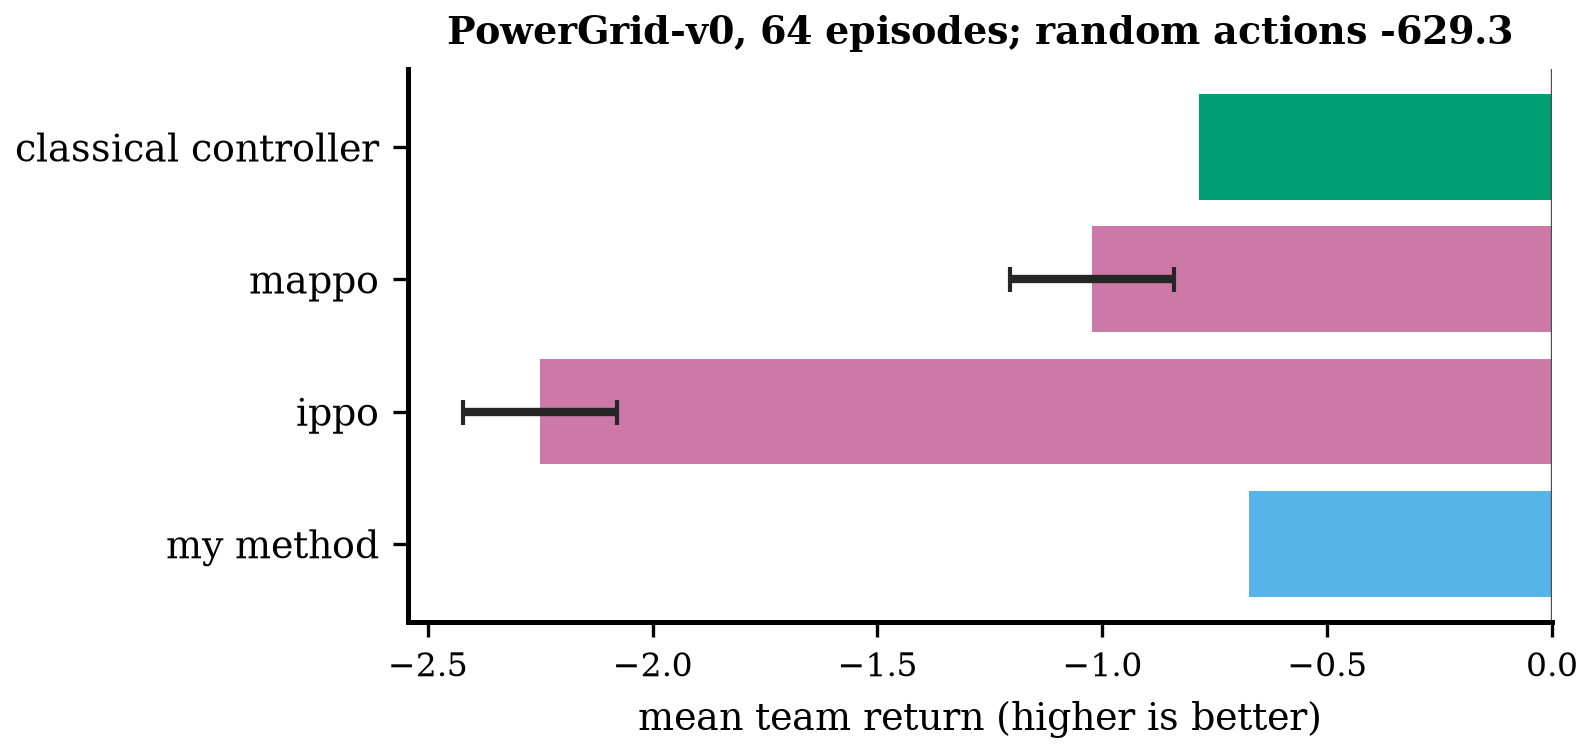
\includegraphics[width=\columnwidth]{figures/baseline_comparison.png}
  \caption{Output of \file{examples/algorithms/baseline_comparison.py}: mean
    return on 64 shared evaluation episodes (seed 1); error bars are the
    standard deviation over two training seeds.}
  \label{fig:compare}
\end{figure}

% ===========================================================================
\section{Engineering and Reproducibility}\label{sec:engineering}
% ===========================================================================

The distribution installs with \code{pip} from the repository, supports
Python 3.9 to 3.13 and needs only NumPy, SciPy, matplotlib, Gymnasium and
PyYAML; PyTorch, pymunk/pygame
and video export are optional extras loaded on first use. {\NumTests} tests
cover the Gymnasium contract of every environment, the equivalence of single
and batched simulation, seeded determinism, the controllers, the wrappers and
the learning baselines, and run in continuous integration on Python~3.9 to
3.13 together with smoke tests of the examples. Rendering works headless,
episodes export to GIF, MP4 or \code{.npz} trajectories, and a handbook
documents the model equations, observation layouts and parameters of every
environment. The distribution also contains small research utilities
(publication-quality plotting, PyTorch building blocks and experiment
parameter management) that are outside the scope of this paper.

% ===========================================================================
\section{Limitations and Conclusion}
% ===========================================================================

The environments are compact models: the grid is lossless and Kron-reduced,
the platoon drives on a single lane, and the robots move in the plane. They
simulate on the CPU with NumPy (the Kuramoto family also on PyTorch), which
suits many small training runs better than accelerator-scale training. The
learning baselines are reference implementations with feed-forward networks
and presets tuned for short budgets rather than for peak performance.

\texttt{env\_lib} offers networked control problems with physical meaning, one
interface, fast batched simulation, and for every task both a classical
controller and learned baselines to compare against. We hope it helps new
MARL methods for networked systems to be measured against the designs that
engineers deploy.

\bibliography{references}
\bibliographystyle{plainnat}

% ===========================================================================
\newpage
\appendix
\onecolumn
\section{Observation Layouts and Actions}\label{app:layouts}

\begin{table}[h]
  \caption{Per-agent observation rows and actions of the continuous
    environments (\code{env.observation\_layout} gives the column of every
    feature; all features are scaled to order one).}
  \label{tab:layouts}
  \centering\small
  \begin{tabular}{@{}>{\raggedright}p{2.6cm}>{\raggedright}p{9.1cm}>{\raggedright\arraybackslash}p{4.4cm}@{}}
    \toprule
    Environment & Observation row of agent $i$ & Action of agent $i$ \\
    \midrule
    PowerGrid-v0 & frequency deviation, rate of change of frequency, disturbance,
      exported power, previous action, mean and maximum neighbour frequency
      deviation, mean neighbour action, capacity, inertia &
      power injection in $[-u_{\max,i}, u_{\max,i}]$ \\
    Platoon-v0 & spacing error, relative speed, speed, acceleration, and the
      communicated predecessor, leader and follower quantities available under
      the V2V topology (with availability flags) &
      acceleration command in $[a_{\min}, a_{\max}]$ \\
    Consensus-v0, Formation-v0 & own position, velocity and formation offset,
      and the offset-corrected relative positions of the neighbours in a fixed
      number of slots & velocity or acceleration in $[-u_{\max}, u_{\max}]^2$ \\
    AJLATT-v0 & target belief relative to the robot (position, heading,
      velocity) and its covariance trace, neighbour robots, the closest
      obstacle, own pose belief and its covariance trace &
      linear velocity in $[0, 2]$\,m/s, angular velocity in $[-\pi/4, \pi/4]$ \\
    \bottomrule
  \end{tabular}
\end{table}

\section{All Presets}\label{app:presets}

\begin{table}[h]
  \caption{All 17 presets (\file{benchmarks/benchmark_marl.py}; training
    seed 0, evaluation on 64 episodes with seed 1, CPU seconds of training on
    one core).}
  \label{tab:presets}
  \centering\small
  \begin{tabular}{@{}llrrrrr@{}}
    \toprule
    Method & Environment & Env steps & Time [s] & Random & Trained & Controller \\
    \midrule
    IPPO & PowerGrid-v0 & 200,704 & 69 & $-629.3$ & $-2.37$ & $-0.79$ \\
    IPPO & Platoon-v0 & 450,560 & 88 & $-5{,}350$ & $-84.8$ & $-46.4$ \\
    IPPO & Consensus-v0 & 401,408 & 83 & $-18{,}041$ & $-1{,}550$ & $-1{,}518$ \\
    IPPO & LineMsg-v0 & 100,800 & 26 & 43.2 & 95.0 & 95.0 \\
    MAPPO & PowerGrid-v0 & 251,904 & 106 & $-629.3$ & $-0.89$ & $-0.79$ \\
    MAPPO & Platoon-v0 & 450,560 & 102 & $-5{,}350$ & $-65.0$ & $-46.4$ \\
    MAPPO & Consensus-v0 & 401,408 & 96 & $-18{,}041$ & $-1{,}586$ & $-1{,}518$ \\
    MAPPO & LineMsg-v0 & 100,800 & 26 & 43.2 & 95.0 & 95.0 \\
    MADDPG & PowerGrid-v0 & 64,000 & 70 & $-629.3$ & $-5.69$ & $-0.79$ \\
    MADDPG & Consensus-v0 & 96,000 & 72 & $-18{,}041$ & $-1{,}681$ & $-1{,}518$ \\
    MATD3 & PowerGrid-v0 & 64,000 & 87 & $-629.3$ & $-5.63$ & $-0.79$ \\
    MATD3 & Consensus-v0 & 96,000 & 83 & $-18{,}041$ & $-1{,}737$ & $-1{,}518$ \\
    IQL & LineMsg-v0 & 25,008 & 9 & 43.2 & 95.0 & 95.0 \\
    VDN & LineMsg-v0 & 25,008 & 10 & 43.2 & 95.0 & 95.0 \\
    VDN & WirelessComm-v1 & 120,000 & 74 & 139.2 & 338.0 & 339.6 \\
    QMIX & LineMsg-v0 & 25,008 & 16 & 43.2 & 95.0 & 95.0 \\
    QMIX & WirelessComm-v1 & 100,000 & 101 & 139.2 & 319.1 & 339.6 \\
    \bottomrule
  \end{tabular}
\end{table}

\section{Reproducing the Numbers}\label{app:repro}

From the root of a clone of the repository (\repo):
\begin{lstlisting}[language=bash]
pip install -e ".[all]"
python benchmarks/benchmark_vector.py              # Table (*\ref{tab:throughput}*), Figure (*\ref{fig:throughput}*)
python benchmarks/benchmark_baselines.py           # Table (*\ref{tab:controllers}*)
python benchmarks/benchmark_marl.py --markdown     # Tables (*\ref{tab:marl}*) and (*\ref{tab:presets}*)
python examples/algorithms/marl_training_demo.py   # Figure (*\ref{fig:curves}*)
python examples/algorithms/baseline_comparison.py  # Figure (*\ref{fig:compare}*)
\end{lstlisting}
All numbers were measured on one core of an Intel Xeon at 2.8\,GHz with
\code{OMP\_NUM\_THREADS=1} and one PyTorch thread; training runs are
deterministic for a given seed, thread count and software stack.

\end{document}
